%%%%%%%%%%%%%%%%%%%%%%%%%%%%%%%%%%%%%%%%%
% Journal Article
% LaTeX Template
% Version 1.3 (9/9/13)
%
% This template has been downloaded from:
% http://www.LaTeXTemplates.com
%
% Original author:
% Frits Wenneker (http://www.howtotex.com)
%
% License:
% CC BY-NC-SA 3.0 (http://creativecommons.org/licenses/by-nc-sa/3.0/)
%
%%%%%%%%%%%%%%%%%%%%%%%%%%%%%%%%%%%%%%%%%

%----------------------------------------------------------------------------------------
%	PACKAGES AND OTHER DOCUMENT CONFIGURATIONS
%----------------------------------------------------------------------------------------

\documentclass[twoside]{article}

\usepackage{graphics}
\usepackage{graphicx}
\usepackage{wrapfig}
\usepackage{multicol}

\usepackage[T1]{fontenc} % Use 8-bit encoding that has 256 glyphs
\usepackage[utf8]{inputenc}

\usepackage[hmarginratio=1:1,top=32mm,columnsep=20pt]{geometry} % Document margins
\usepackage[hang, small,labelfont=bf,up,textfont=it,up]{caption} % Custom captions under/above floats in tables or figures
\usepackage{booktabs} % Horizontal rules in tables
\usepackage{float} % Required for tables and figures in the multi-column environment - they need to be placed in specific locations with the [H] (e.g. \begin{table}[H])
\usepackage{hyperref} % For hyperlinks in the PDF

\usepackage{lettrine} % The lettrine is the first enlarged letter at the beginning of the text
\usepackage{paralist} % Used for the compactitem environment which makes bullet points with less space between them

\usepackage{abstract} % Allows abstract customization
\renewcommand{\abstractnamefont}{\normalfont\bfseries} % Set the "Abstract" text to bold
\renewcommand{\abstracttextfont}{\normalfont\small\itshape} % Set the abstract itself to small italic text

\usepackage{fancyhdr} % Headers and footers
\pagestyle{fancy} % All pages have headers and footers
\fancyhead{} % Blank out the default header
\fancyfoot{} % Blank out the default footer
\fancyhead[C]{Améliorations d'images sous-marines. Rapport de Projet} % Custom header text
\fancyfoot[RO,LE]{\thepage} % Custom footer text

%----------------------------------------------------------------------------------------
%	TITLE SECTION
%----------------------------------------------------------------------------------------

\title{\vspace{-15mm}\fontsize{24pt}{10pt}\selectfont\textbf{Amélioration d'images sous-marines}} % Article title

\author{
\large
\textsc{Jean Caillé, Florian Denis}\\[2mm] % Your name
\normalsize Télécom ParisTech - SI241 \\ % Your institution
\normalsize \href{mailto:jean.caille@polytechnique.edu}{jean.caille@polytechnique.edu} - \href{mailto:florian.denis@polytechnique.edu}{florian.denis@polytechnique.edu}  % Your email address
\vspace{-5mm}
}
\date{}

%----------------------------------------------------------------------------------------

\begin{document}

\maketitle % Insert title

\thispagestyle{fancy} % All pages have headers and footers

%----------------------------------------------------------------------------------------
%	ABSTRACT
%----------------------------------------------------------------------------------------

\vspace{0.5cm}
\begin{abstract}
Les images sous-marines sont par définition acquises dans un environnement où les conditions de visibilité sont particulièrement mauvaises. Ainsi, les images obtenues par des appareils classiques sont fortement dégradées. L'hétérogénéité du milieu, la diffusion de la lumière par les particules en suspension et la non-transparence de l'eau contribuent chacun à une prise de vue s'éloignant de la réalité. L'article que nous avons étudié montre qu'il est possible de corriger ces dégradations dans certains cas, en utilisant des hypothèses minimes quant à la scène observée. Cette méthode est de plus applicable à un grand nombre d'exemples car elle ne nécessite qu'une image en entrée.\\
Nous avons étudié, implémenté et mesuré les performances de la méthode proposée par les auteurs de l'article. Dans ce rapport, nous nous attacherons à décrire d'une part la technique employée, ainsi que les outils utilisés pour l'implémentation. Nous analyserons ensuite nos résultats et les comparerons avec ceux obtenus par les auteurs. Finalement, nous tenterons de suggérer des améliorations à cette méthode.\\

\end{abstract}

%----------------------------------------------------------------------------------------
%	ARTICLE CONTENTS
%----------------------------------------------------------------------------------------

\section{Introduction et Motivation}
Aujoud'hui, le grand public commence à s'équiper d'appareils photos résistants à l'eau (GoPro, ...). Les images acquises dans ces conditions difficiles sont souvents dégradées. Toutefois, ce même matériel est suffisement sensible pour permettre la restauration des images, permettant alors d'améliorer grandement la qualité des images rendues.\\
Nous avons choisi d'effectuer ce projet car les résultats promis par l'article et la description qui en était faite nous semblait intéressants. Plusieurs concepts variés, très utilisés en images sont introduits (balance des blancs et Gray-World, fusion par pyramide, ...). De plus, les techniques utilisées dans le papier sont applicables à de nombreux problèmes de restauration d'images, en particulier les images dégradées par un brouillard ou par la polution aérienne. Finalement, ce projet nous permettait de tester notre implémentation dans des cas réels (typiquement : des images sous-marines trouvées sur internet). En effet, contrairement à certains projets ou les données d'entrées sont nombreuses, ou dans un format particulier, la technique décrite dans l'article peut s'appliquer aux photos individuelles.\\
L’article propose un post-traitement basé sur la fusion d’images afin d’améliorer la qualité de la prise de vue. Les applications d’un tel traitement sont nombreuses, tant pour l’affichage et la visualisation de ces images que pour des problématiques de visions plus intéressantes (tel l’extraction de points clés, la détection de contours et la reconnaissance de forme).\\

%------------------------------------------------

\section{Méthode}

La méthode décrite par l’article consiste en la fusion de deux images générées (appelées images d'entrées) à partir de l’image initiale. Les auteurs supposent que les dégradations de la prise de vue sous-marine sont dues d’une part à la balance des couleurs ainsi que les contrastes de la scène. Ainsi les deux images qui seront fusionnées sont chacune créées afin de résoudre un de ces problèmes.\\

%---------------------------------------------------> SUB SECTION Balance des blancs
\subsection{Balance des blancs}

\begin{figure}[H]
  \centering
  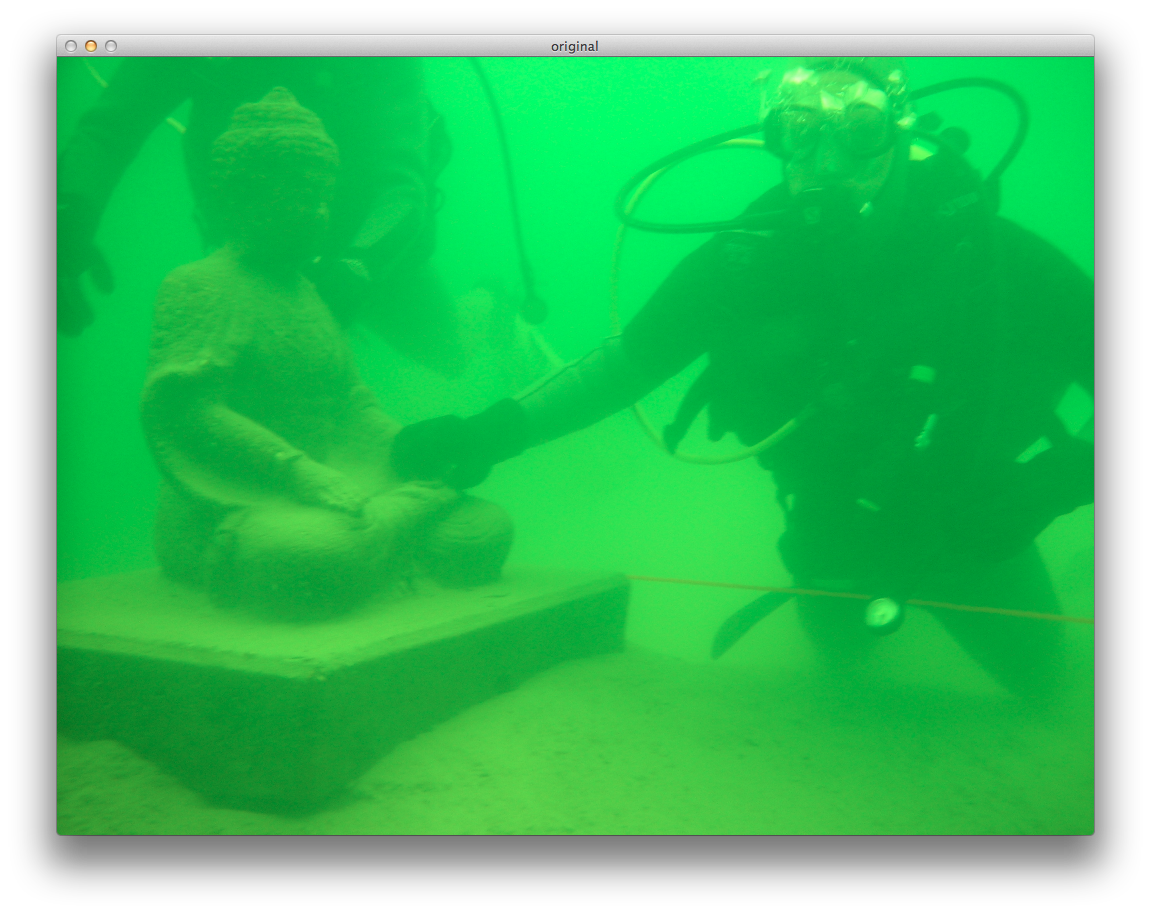
\includegraphics[width=0.75\textwidth]{Support/input.png}
  \caption{caption}
\end{figure}

La première image du processus de fusion est créée afin de corriger les problèmes de balance de blancs qui existent lors des prises de vue sous-marines. Comme nous pouvons le voir sur la figure, les informations de couleurs semblent à première vue être perdues.\\
Nous pouvons toutefois en post-traitement corriger la balance des blancs. L'article suggère plusieurs méthodes, mais aucune n'est décrite en particulier. Nous avons donc choisi d'implémenter la méthode dite de \emph{Gray-World}. L'idée sous-jacente de cette technique est de trouver l'\emph{illuminant} $i$, c'est à dire la couleur de la lumière éclairant la scène. Une fois $i$ trouvé, nous pouvons "corriger" cette couleur à l'ensemble des pixels de la scène pour retrouver les couleurs réelles (\emph{i.e.} en lumière blanche).\\
L'hypothèse \emph{Gray-World} suppose que la couleur moyenne d'une scène est un niveaux de gris $g$. Ainsi si on mesure $m$ la moyenne réelle des pixels de l'image : $$m = \frac{1}{N}\sum_{x \in image}I(x)$$ On peut calculer $g$ comme $$g = \frac{m_r + m_g + m_b}{3}$$ L'article suggère une correction de la luminosité de scène pour compenser la perte de luminosité due au milieu $$g' = 0.5 + \lambda g$$ où $\lambda$ est un paramètre dont la valeur recommandée par les auteurs est $0.2$. On en déduit alors la couleur de l'illuminant $$ i = \frac{m}{g}$$ Finalement, on corrige la couleur de la scène en modifiant la valeur du pixel $$I(x) = \frac{I(x)}{i}$$\\
Nous avons ainsi corrigé l'image de telle sorte que la somme des couleurs soit effectivement une nuance de gris. L'image obtenu sera la première entrée du processus de fusion.

\begin{figure}[H]
  \centering
  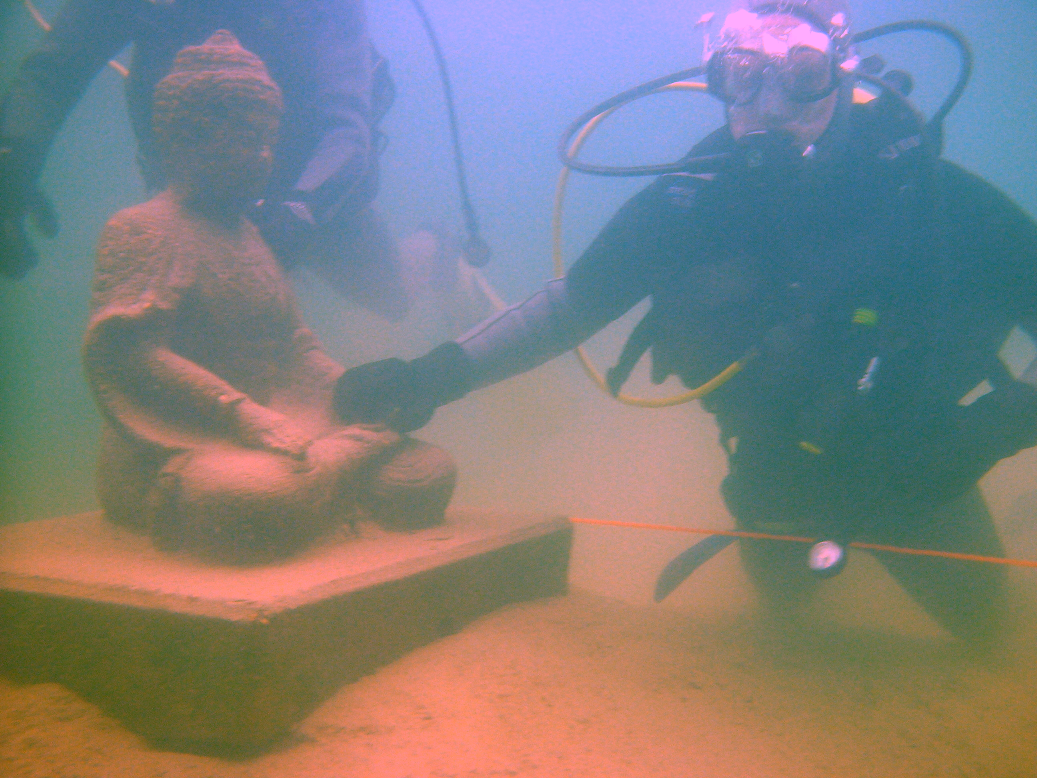
\includegraphics[width=0.75\textwidth]{Support/color.png}
  \caption{L'image dont les couleurs ont été corrigées. On note la présence d'une tache rouge sur le visage de l'homme de droite, peut être due à un mauvais paramètre $\lambda$.}
\end{figure}

%---------------------------------------------------> SUB SECTION Amélioration du Contraste
\subsection{Amélioration du Contraste}
La seconde entrée du processus de fusion est quand à elle créée pour corriger les problèmes de contrastes dus à la diffusion de la lumière dans le milieu aquatique. Elle est obtenue à partir de l'image où les couleurs ont été corrigées. Elle est obtenue en deux étapes : réduction du bruit puis amélioration du constraste.\\
La réduction du bruit est effectuée à l'aide d'un simple filtre bilatéral. Ce filtre non linéaire remplace l'intensité de chaque pixel par une moyenne pondérée des pixels avoisinants, où les poids dépendent à la fois de la distance au pixel central, mais également de la différence d'intensité entre les pixels considérés. Ce filtre a la propriété de conserver les contours tout en supprimant correctement le bruit. Il est important de noter que si l'article conseille un débruitage cohérent dans le temps (pouvant donc s'appliquer à la vidéo), cela n'est pas nécessaire pour les applications à des images simples.\\
Il existe de nombreuses méthodes permettant de réhausser le contraste de l'image, en particulier la méthode de \emph{Local Adaptative Histogram Equalization} qui égalise localement des histogrammes, c'est-à-dire une transformation locale du constraste basée sur le voisinage du pixel. Contrairement à une méthode globale, on ne court pas le risque de saturer l'image tout en gardant une plage dynamique maximum. Toutefois, il est important de noter que cette technique est peut sensiblement augmenter la quantité de bruit. Si le filtre bilatéral appliqué n'est pas assez puissant, il peut être nécessaire d'employer une technique plus robuste pour augmenter le constraste. Une solution consiste à employer une méthode similaire nommée \emph{Constrast Limited Adaptative Histogram Equalization (CLAHE)}. Dans cette méthode, le contraste est limité, et les pics de l'histogramme sont redistribués uniformément.

\begin{figure}[]
  \centering
  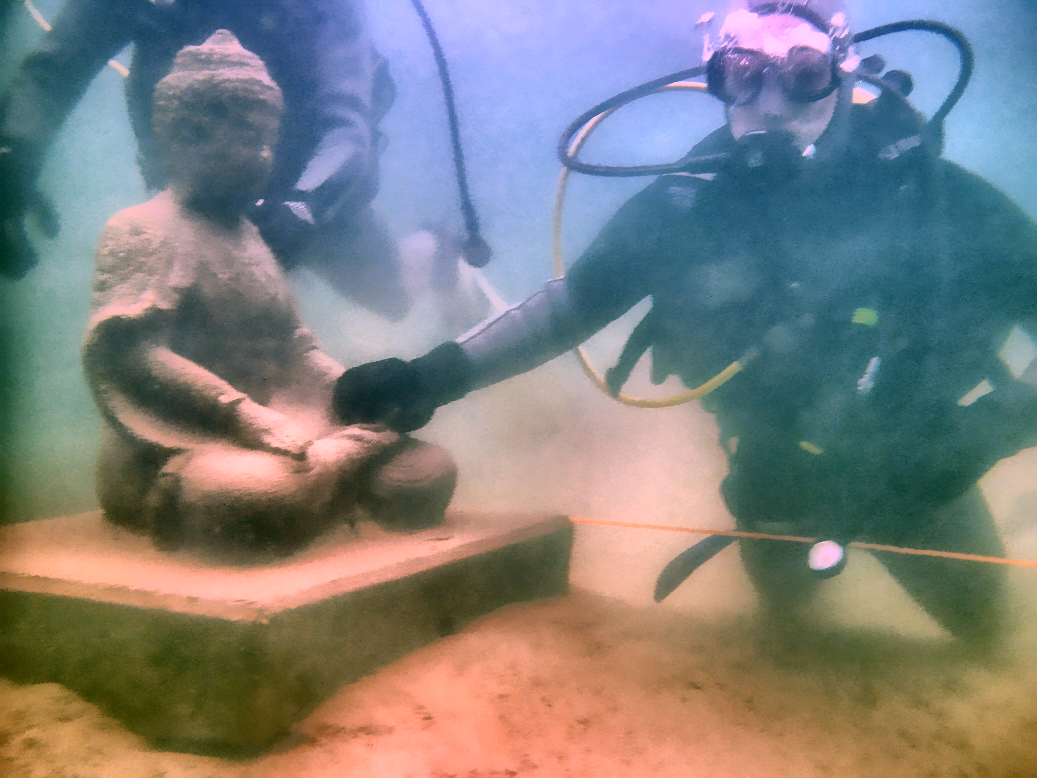
\includegraphics[width=0.75\textwidth]{Support/contrast.png}
  \caption{L'image après amélioration du contraste}
\end{figure}

%---------------------------------------------------> SUB SECTION Poids de fusions
\subsection{Poids de fusions}
Une fois les deux entrées générées, il est nécessaire de les fusionner de manière intelligente. Une simple moyenne des images (fusion naïve) n'est pas adaptée, en effet, sur certaines zones (contours, zones visuellement proéminentes) il est nécessaire de faire ressortir le contraste (et donc l'entrée numéro 2) au détriment des couleurs, alors que dans les zones constantes (aplats de couleur), il vaut mieux mettre en avant la correction de couleur. La fusion va donc s'effectuer en fonction d'un ou plusieurs poids, qui dénotterons l'importance que l'on souhaite appliquer à chaque image d'entrée dans l'image résultante, et ce pour tous les pixels considérés. 

%------------------------------------------------------------> SUB SUB SECTION Poid 1
\subsubsection{Poids Laplacien}

Il se calcul en appliquant un filtre laplacien sur chaque entrées du filtre. Il est censé mettre en valeur les contours et zones texturées, mais est peu adapté aux problèmes de restaurations d'images sous-marines, car il ne fait pas la différence entre zones de luminosité constante et zones de luminosité légèrement croissante (ou décroissante)

\begin{figure}[]
  \centering
  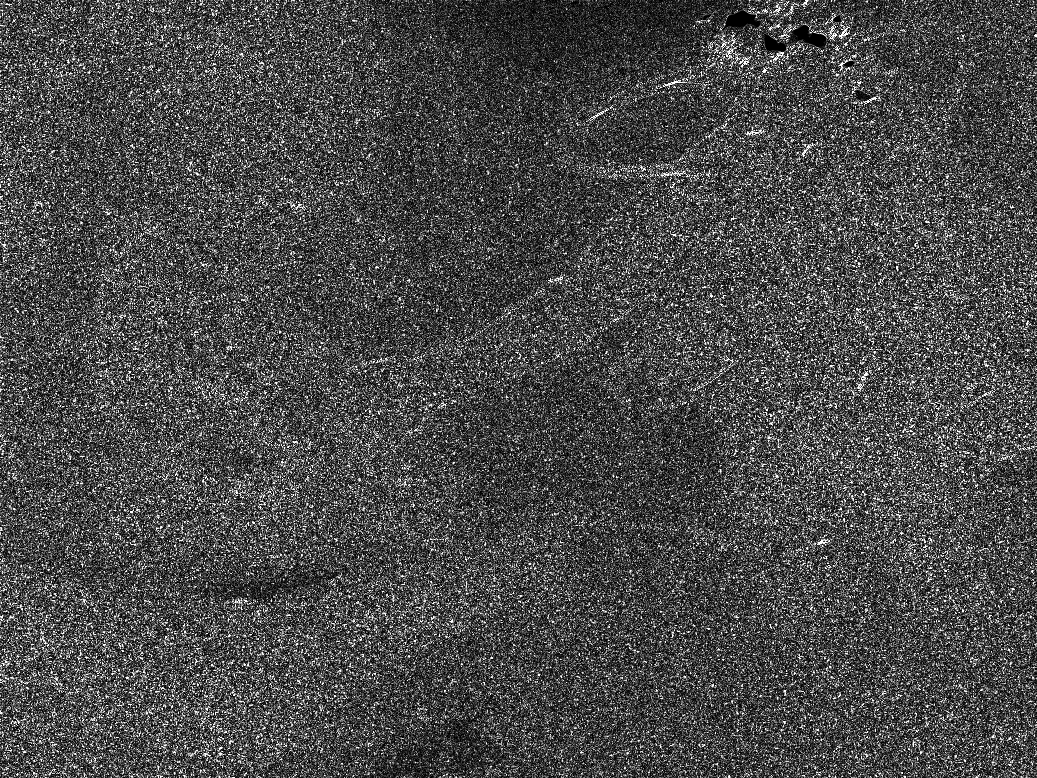
\includegraphics[width=0.45\textwidth]{Support/laplacian.png}
  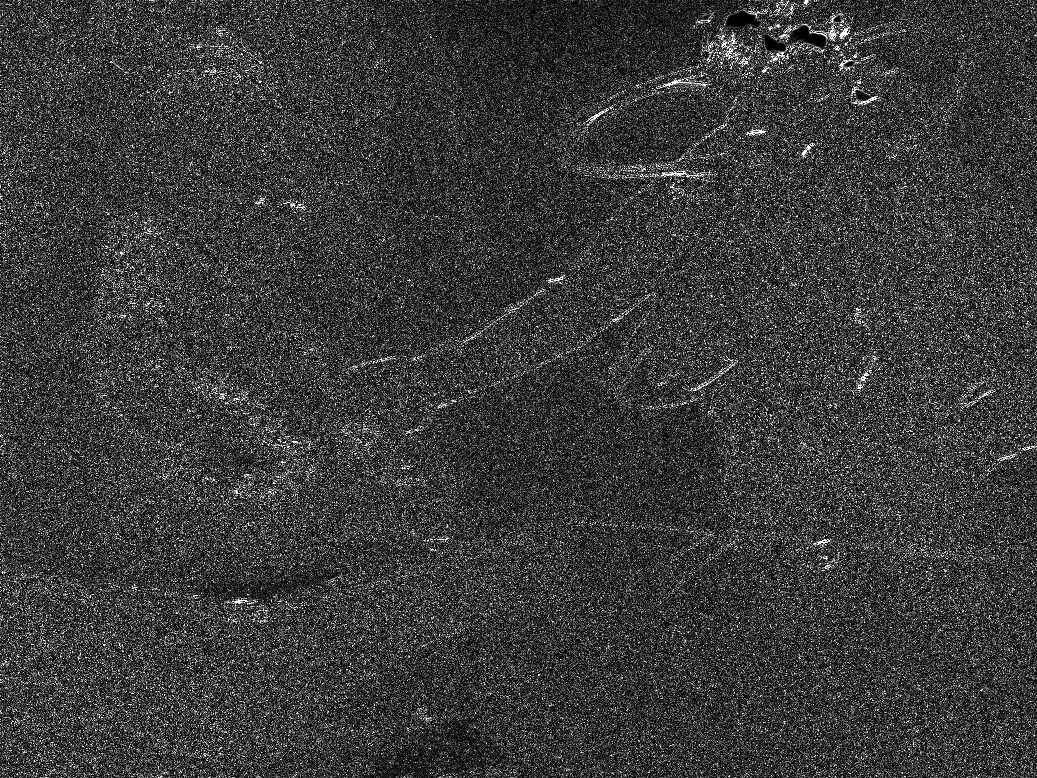
\includegraphics[width=0.45\textwidth]{Support/lc.png}

  \caption{Poids laplacien et Poids de contraste local. Les valeurs des poids ont été multipliés par 5 pour les rendres visibles sur la figure, ce qui explique la forte présence de bruit}
\end{figure}

%------------------------------------------------------------> SUB SUB SECTION Poids 2
\subsubsection{Poids de Contraste Local}

Ce poids a été créé pour mettre en avant les zones contrastées. Il se calcul en chaque pixel par la différence de la valeur de l'image I avec la valeur de I filtré par un passe-bas : $$ W_{LC}(x,y) = \|I(x,y) - I_{f}(x,y)\| $$
L'article recommande l'utilisation pour le filtre passe-bas d'un noyeau binomial séparable de taille $5$ x $5$. Ce filtre est en effet une bonne approximation d'une Gaussienne, tout en restant algorithmiquement peu couteux à calculer.

%------------------------------------------------------------> SUB SUB SECTION Poids de Saillance
\subsubsection{Poids de Saillance}
Le poids de saillance cherche à mettre en valeur les objets visuellement proéminants qui peuvent exister dans une scène sous-marine. Une technique pour trouver la saillance d'un point est de comparer sa valeur avec une moyenne des valeurs des pixels l'entourant. Ce comportement est similaire au concept biologique de \emph{center-surround constrast}, ou contraste centre-contour. Toutefois, l'article précise que ce poids favorise les zones lumineuses, et pour protéger les tons moyens, les auteurs suggèrent l'utilisation du poids d'exposition.

\begin{figure}[]
  \centering
  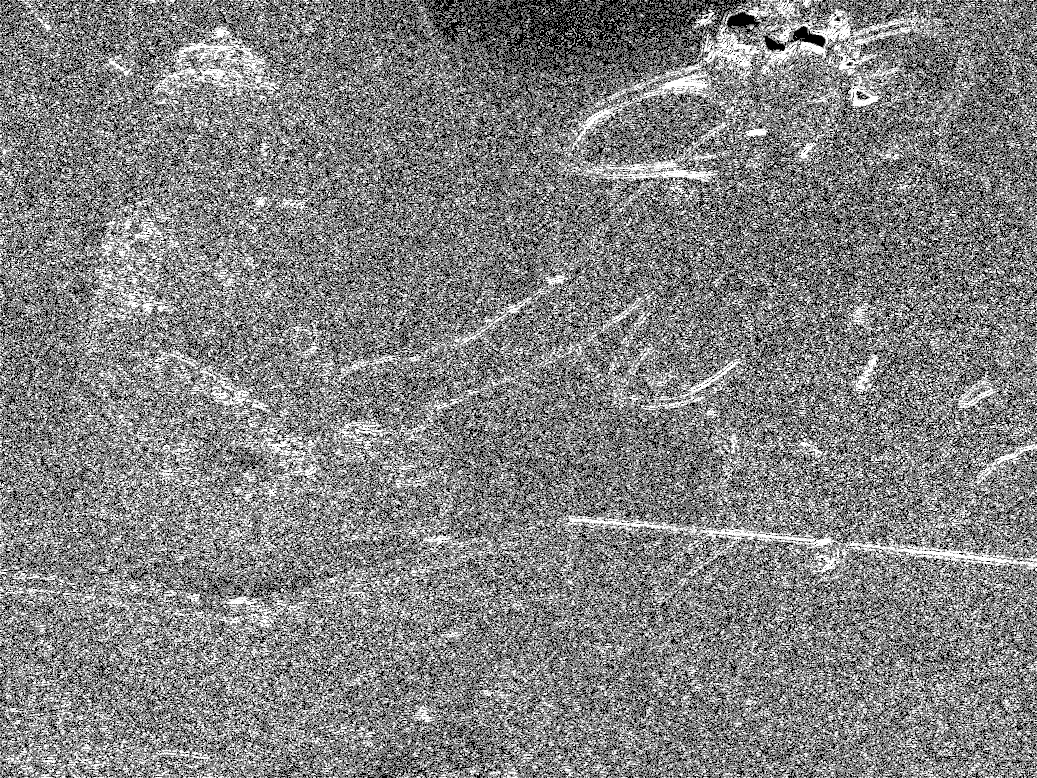
\includegraphics[width=0.45\textwidth]{Support/saliency.png}
  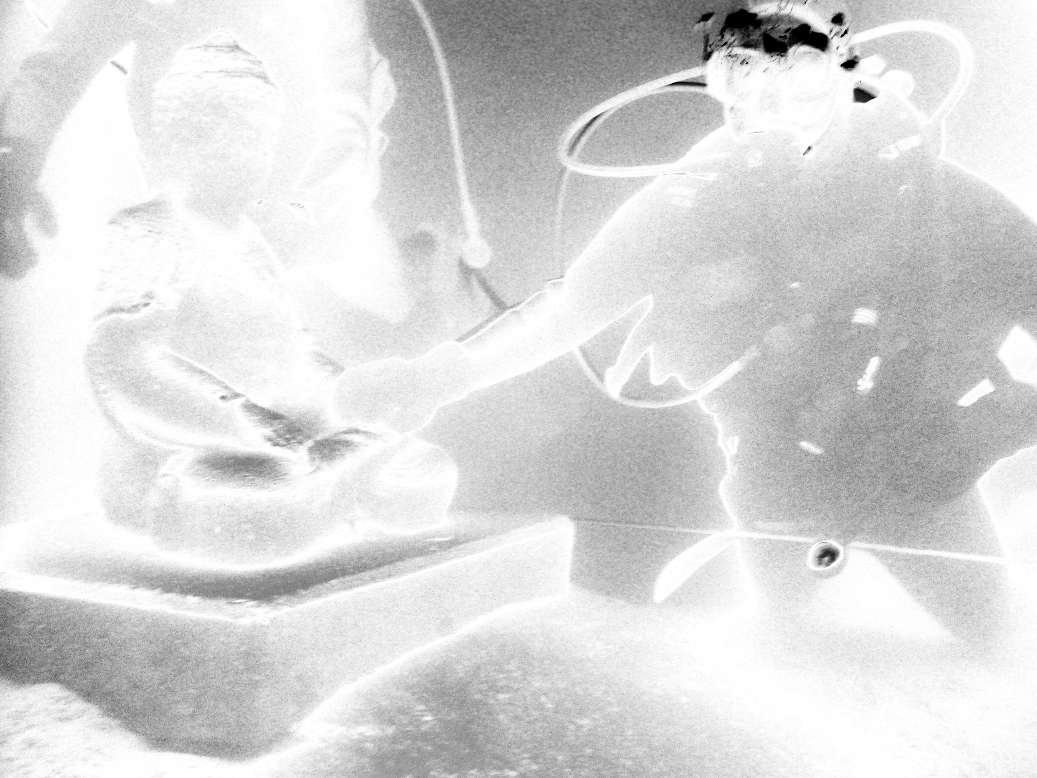
\includegraphics[width=0.45\textwidth]{Support/exposedness.png}
  \caption{Poids de Saillance et poids d'exposition. Les valeurs des poids ont été multipliés par 5 pour les rendres visibles sur la figure, ce qui explique la forte présence de bruit}
\end{figure}

%------------------------------------------------------------> SUB SUB SECTION Poids d'exposition
\subsubsection{Poids d'exposition}
Cette carte de poids cherche à estimer si le pixel considéré est bien exposé, i.e. si sa luminosité est proche de la valeur moyenne $0.5$. On utilise ensuite une gaussienne pour obtenir la valeur du poids $$W_{exp}(x,y) = \exp{-\frac{(I(x,y) - 0.5)^2}{2\sigma^2}}$$

%------------------------------------------------------------> SUB SUB SECTION Normalisation des poids
 \subsubsection{Normalisation des poids}
Plusieurs poids sont suggérés, mais seulement deux (un par entrée) sont utilisés dans le processus de fusion. Pour normaliser la contribution de chaque image, on modifie les poids de sorte que la somme des deux cartes de poids soit constante et égale à $1$. Cette modification est uniquement locale, et ne dépend que de la valeur des poids au pixel considéré.

%---------------------------------------------------> SUB SECTION Fusion par pyramide Laplacienne
\subsection{Fusion par pyramide Laplacienne}
L'article souligne qu'une fusion naïve des deux images, même en utilisant les poids, donne des résultats visuellement peu plaisants, avec par exemple l'apparition de halos ou une distortion des couleurs. Les auteurs suggèrent donc l'utilisation d'une méthode classique de fusion d'image : la fusion Laplacienne, ou fusion par pyramide Laplacienne. Cette fusion s'effectue dans un espace échelle, et l'image finale est obtenue en combinant les deux images d'entrées et les deux poids dans cet espace échelle. En particulier, on construit des pyramides Laplaciennes pour les images d'entrées, tandis que les poids sont utilisés pour créer des pyramides gaussiennes. Finalement, les contributions de chaque niveau de la pyramide sont sommées pour obtenir l'image finale.\\

%---------------------------------------------------> SUB SECTION Pyramide Gaussienne
\subsection{Pyramide Gaussienne}
Une pyramide gaussienne est une représentation de l'image sur plusieurs niveaux de résolutions. Elle permet à l'algorithme de fusion de considérer l'image comme une réunion échelles de détails, du plus fin au plus grossier. Pour passer descendre d'un niveau dans la pyramide, on convolue l'image par un filtre gaussien (passe-bas), puis on divise la résolution de l'image par deux.

\begin{figure}
  \centering
  \vspace{0.1cm}
  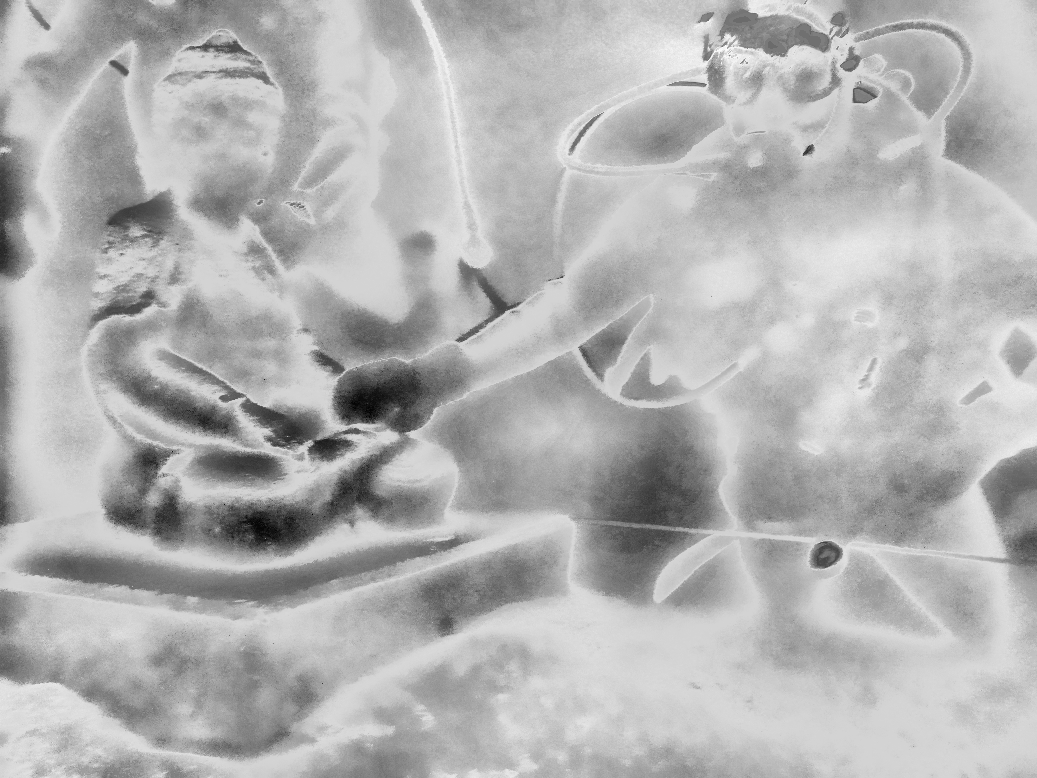
\includegraphics[width=0.4\textwidth]{Support/gaussian0.png}
  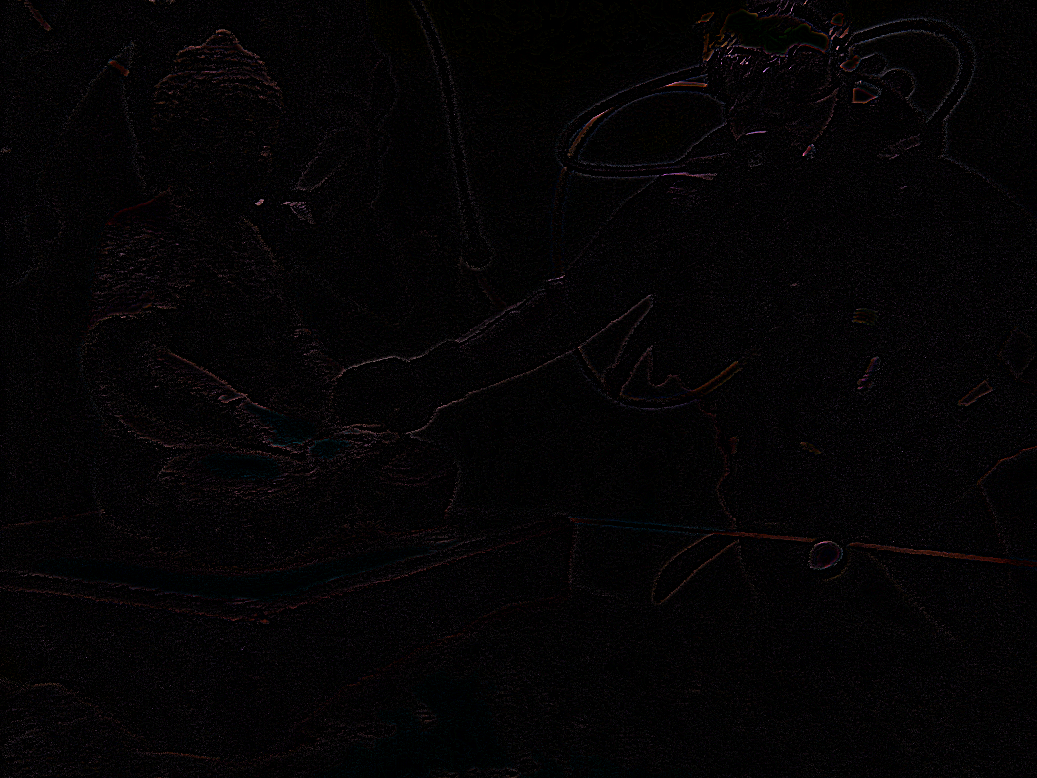
\includegraphics[width=0.4\textwidth]{Support/laplacian0.png}\\
  \vspace{0.1cm}
  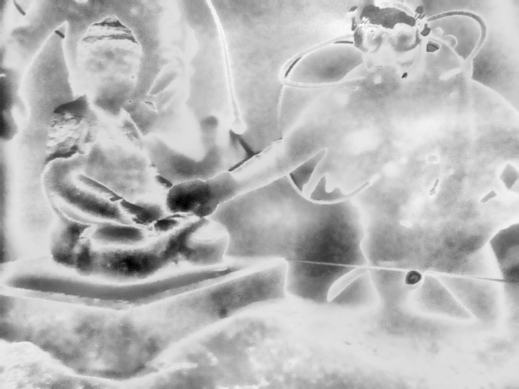
\includegraphics[width=0.4\textwidth]{Support/gaussian1.png}
  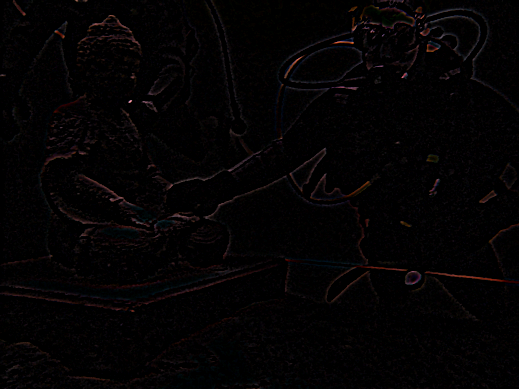
\includegraphics[width=0.4\textwidth]{Support/laplacian1.png}\\
  \vspace{0.1cm}
  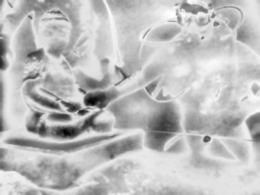
\includegraphics[width=0.4\textwidth]{Support/gaussian2.png}
  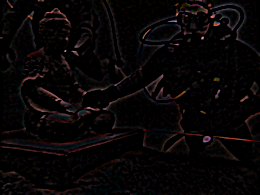
\includegraphics[width=0.4\textwidth]{Support/laplacian2.png}\\
  \vspace{0.1cm}
  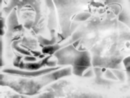
\includegraphics[width=0.196\textwidth]{Support/gaussian3.png}
  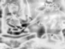
\includegraphics[width=0.196\textwidth]{Support/gaussian4.png}
  \vspace{0.1cm}
  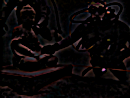
\includegraphics[width=0.196\textwidth]{Support/laplacian3.png}
  
\includegraphics[width=0.196\textwidth]{Support/laplacian4.png}

  \caption{Pyramide gaussienne du poids d'exposition et pyramide laplacienne de l'image d'entrée}
\end{figure}


%---------------------------------------------------> SUB SECTION Pyramide Laplacienne
\subsection{Pyramide Laplacienne}
La pyramide laplacienne est similaire à la pyramide gaussienne, a ceci près que le filtre appliqué avant la réduction de la taille de l'image est un filtre laplacien. Cette technique permet de faire ressortir des contours de plus en plus larges de l'image.

\section{Implémentation}
Nous avons choisi pour l'implémentation de la méthode décrite dans l'article le language \texttt{C++}, et utilisé la librairie de vision par ordinateur open-source \texttt{OpenCV}. Cette librairie fournie de nombreux outils accélerant la mise en place des différentes méthodes décrites par l'article. Le code finale fait en lui même un peu plus de 400 lignes, et est disponible en ligne sur \texttt{\href{http://github.com/jcaille/Submarine}{gihub}}.

%---------------------------------------------------> SUB SECTION Choix effectués
\subsection{Choix effectués}
Comme nous l'avons mentionné, l'article propoe souvent plusieurs méthodes pour arriver au même résultat. Par exemple, la partie concernant la balance des blancs mentionne en particulier l'algorithme \emph{Gray-World}, l'algorithme \emph{Shades-Of-Gray} ainsi que les approches de Finlayson et Trezzi et l'hypothèse de \emph{Gray-Edge}. Nous avons dans ces cas là fait le choix de n'implémenter qu'une des méthodes décrites pour pouvoir arriver le plus vite possible au résultat final, et comparer nos résultats à ceux montrés par les auteurs. Nous avons ainsi choisi d'implémenter celles qui était la plus mise en avant par les auteurs.\\
Nous avons toutefois pris le soin d'implémenter tous les poids décrits par les auteurs, afin de pouvoir comparer leur influence sur le résultat final.

\section{Résultats}
%---------------------------------------------------> SUB SECTION Aspect visuel et comparaison avec l'article
\subsection{Aspect visuel et comparaison avec l'article}

\begin{figure}[H]
  \centering
  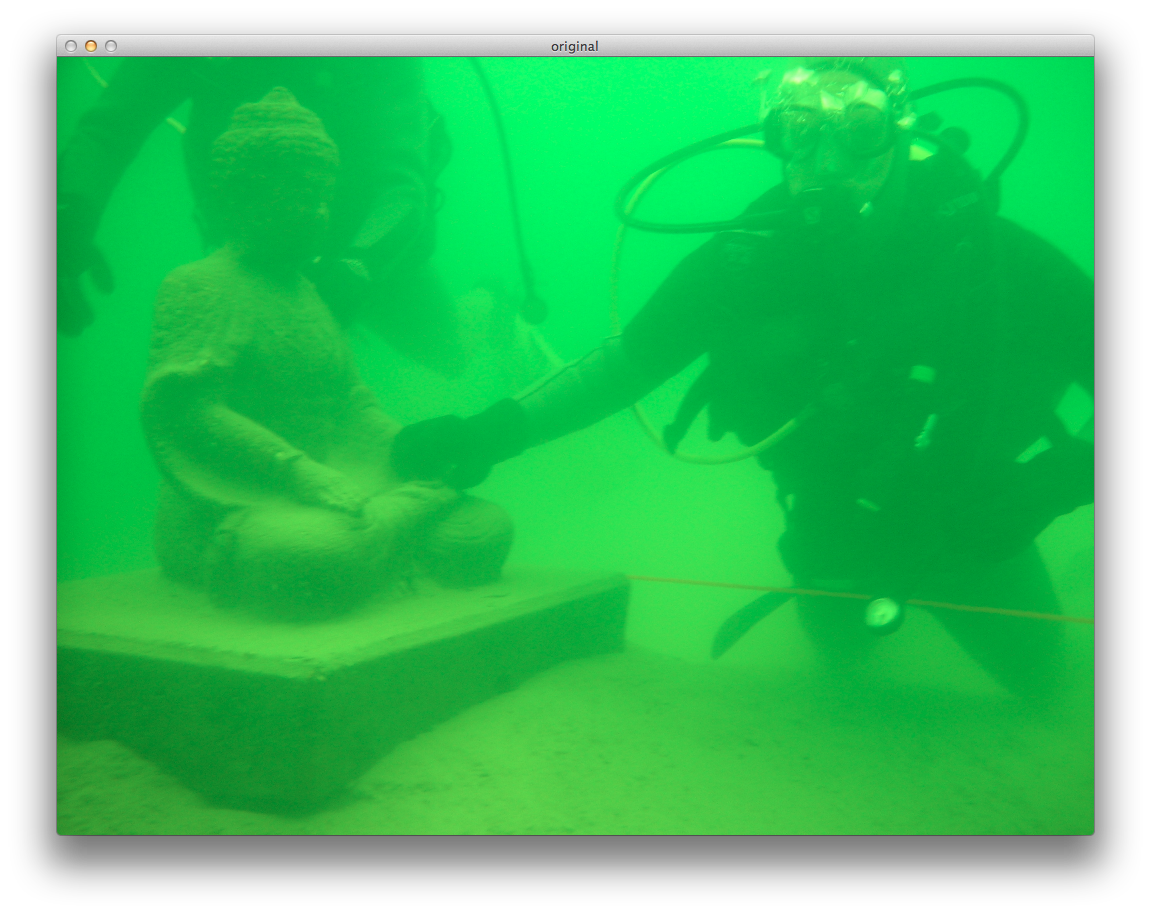
\includegraphics[width=0.45\textwidth]{Support/input.png}
  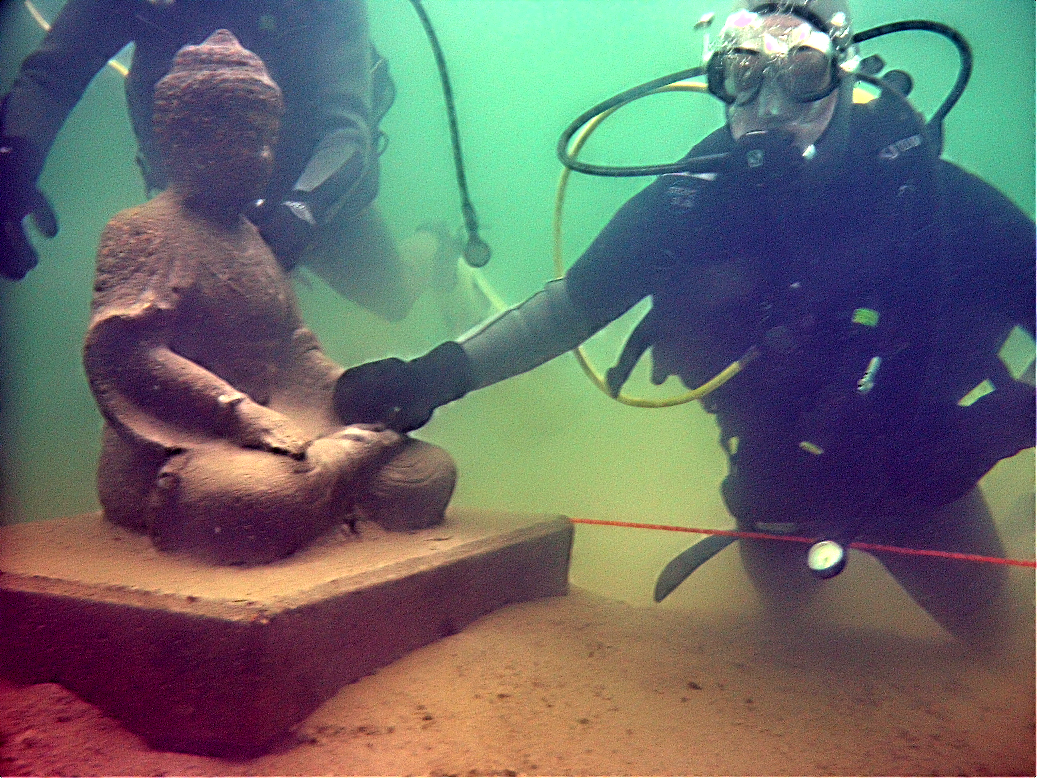
\includegraphics[width=0.45\textwidth]{Support/theirs.png}
  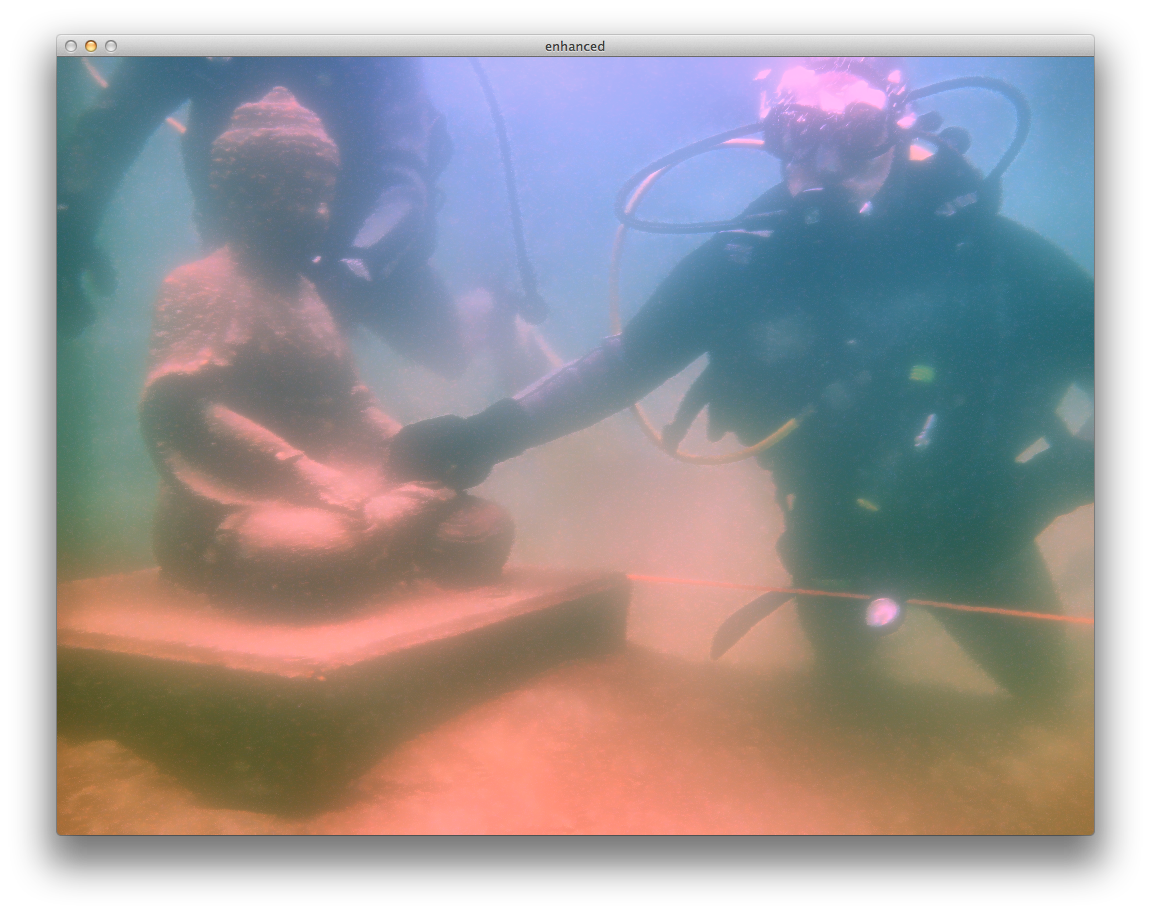
\includegraphics[width=0.55\textwidth]{Support/ours.png}
  \caption{Comparaison des résultats. En haut : L'image d'entrée et les résultats des auteurs. En bas : notre résultat.}
\end{figure}

Nous avons testé notre implémentation sur les différentes images utilisées dans l'article. Nous avons également trouvé sur le site des auteurs leurs résultats en haute définition. Notre implémentation produit des résultats corrects, mais il existe quelques différences avec ceux obtenus par les auteurs de l'article. \\
Tout d'abord, les couleurs dans notre implémentation sont de moins bonne qualité. On voit souvent apparaitre des tâches rouges, et la dynamique de couleur est moins importante. Cela est peut-être du à un mauvais choix du paramètre $\lambda$ (que les auteurs conseillent de fixer à $0.2$), où à un mauvais choix de l'implémentation de l'algorithme de balance des blancs (comme précisé précedemment, plusieurs options étaient mentionnées dans l'article, et aucune n'était clairement mise en avant).\\
Nous observons ensuite un contraste moins important dans nos images, mais également un bruit réduit. Ceci est peut être du à l'utilisation d'un filtre bilatéral pour le débruitage initial, qui limite alors l'augmentation du contraste. Un choix judicieux parmis les différentes combinaisons de poids proposés par les auteurs pourrait également potentiellement améliorer les résultats de ce point de vue.
En conclusion, nous obtenons des résultats comparables, mais de qualité inférieure. Ceci est attendu, car nous n'avons pas tenté d'optimiser pour chaque image les paramètres ($\lambda$, débruitage, poids, ...) pour obtenir le meilleur résultat, mais avons essayé de fixer les paramètres donnant un résultat correct sur chaque image du jeu de test.

%---------------------------------------------------> SUB SECTION Vitesse d'éxecution
\subsection{Vitesse d'exécution}
La vitesse d'exécution est correcte. En moyenne, pour traiter une image de taille 1037x768, l'algorithme nécessite $1.9$ secondes. Nous n'avons ainsi par cherché à optimiser particulièrement la vitesse d'exécution de notre code. Plusieurs améliorations sont possibles à ce niveau. Nous aurions pu utiliser la programmations sur GPU, pour par exemple accélerer la fusion laplacienne ou la mise en place des \emph{CLAHE}. Nous aurions pu également accéléré l'étape de balance des blancs en calculant la valeur de l'illuminant sur une plus petite portion de l'image.

%---------------------------------------------------> SUB SECTION Mesure de la qualité du résultat
\subsection{Mesure de la qualité du résultat}
Si visuellement parlant, les résultats sont satisfaisants, une mesure de la qualité de nos résultats indépendante est nécessaire. Pour cela, l'article évoque que leur technique permet également d'améliorer les résultats d'autres méthodes, tels que la détection et le matching de features. Les auteurs remarquent que peut de points remarquables sont détectés sur les images initiales, mais que de nombreux points de ce types étaits obtenus sur les images corrigées. Nous avons donc voulu mesurer la qualité de nos résultats en comptant le nombres de SURF (\emph{Speeded Up Robust Features}) trouvés sur les images.

\begin{table}[H]
	\centering
    \begin{tabular}{llll}
    \# de SURF : &Init. &Amélioré\\
    \toprule
    DSCN6522     & 33       & 136        & 312 \%     \\
    DSCN6523     & 25       & 66         & 164 \%     \\
    DSCN6532     & 48       & 93         & 94 \%      \\
    DSCN6533     & 22       & 86         & 291 \%     \\
    DSCN6538\_1  & 25       & 60         & 140 \%     \\
    DSCN6539     & 70       & 97         & 39 \%      \\
    DSCN6540     & 27       & 74         & 174 \%     \\
    PICT0400     & 19       & 65         & 242 \%     \\
    PICT0403     & 20       & 47         & 135 \%     \\
    PICT0422     & 260      & 425        & 64 \%      \\
    \toprule
    \textbf{MOYENNE}        & &    & \textbf{165,4\%}      \\
    \end{tabular}
    \caption{Nombre de SURF trouvés avant et après amélioration de l'image par notre implémentation.}
\end{table}

Nous voyons donc qu'en moyenne, 165\% fois plus de points d'intérêts sont détectés après l'amélioration de l'image. Toutefois, ces résultats sont faibles par rapport aux résultats de l'article, où des chiffres de l'ordre de 800\% sont atteints. On peut supposer que la mauvaise amélioration du contraste et de la balance des couleurs dans notre implémentation mène à une moins bonne détection des SURF, qui se basent notamment sur les contours, et la matrice Hessienne, fortement sensible au contraste de l'image.

\section{Ouvertures et Améliorations possibles}
Différentes améliorations sont envisageagles. Tout d'abord, nous pourrions essayer de trouver pourquoi les résultats obtenus avec notre implémentation ne sont pas aussi bon que ceux obtenus par les auteurs de l'article. Il est probable que plusieurs paramètres rentrent sont à prendre en considération, et que certains choix effectués durant l'implémentation n'ont pas été corrects. En outre, plusieurs ouvertures et applications des méthodes présentées dans l'article sont possibles. Comme mentionné par les auteurs, une technique similaire peut être utilisée pour traiter des images dégradées par le brouillard. Nous n'avons pas testé notre implémentation sur de telles images, mais il aurait pu être intéressant de voir quels paramètres étaient les plus adaptés à ce traitement. Nous pourrions également chercher à améliorer l'algorithme et implémenter le débruitage temporel, afin de pouvoir traiter la vidéo en une échelle de temps raisonnable (actuellement, à raison de $2$ secondes par image, le traitement se fait en seulement $60$ fois le temps réel).

%----------------------------------------------------------------------------------------

\end{document}
